% 图 63.3 —— 由 `checks/emit_hand.py` 自动拼出（probe 精测 + prims2 图元分解）
%%
% ⚠ 这是**稿子不是成品**：跑 `checks/checkhand.py 63.3` 看指标 + 看叠合图。
%%
%% ⚠ 待核：
%   · 本图 probe 报出阴影族 1 个 —— **本脚本不生成阴影**（要照原书手写）；prims2 的 strokes 里可能含阴影线，核对时留意别画重
%   · 可疑字形 4 项（空心圈 ⊙ 常被认成字母 o）—— 见文件末
%%
\documentclass[12pt]{standalone}
\usepackage{fontspec}
\setsansfont{Arial}
\newfontfamily\mfallback{DejaVu Sans}
\usepackage{tikz}
\begin{document}
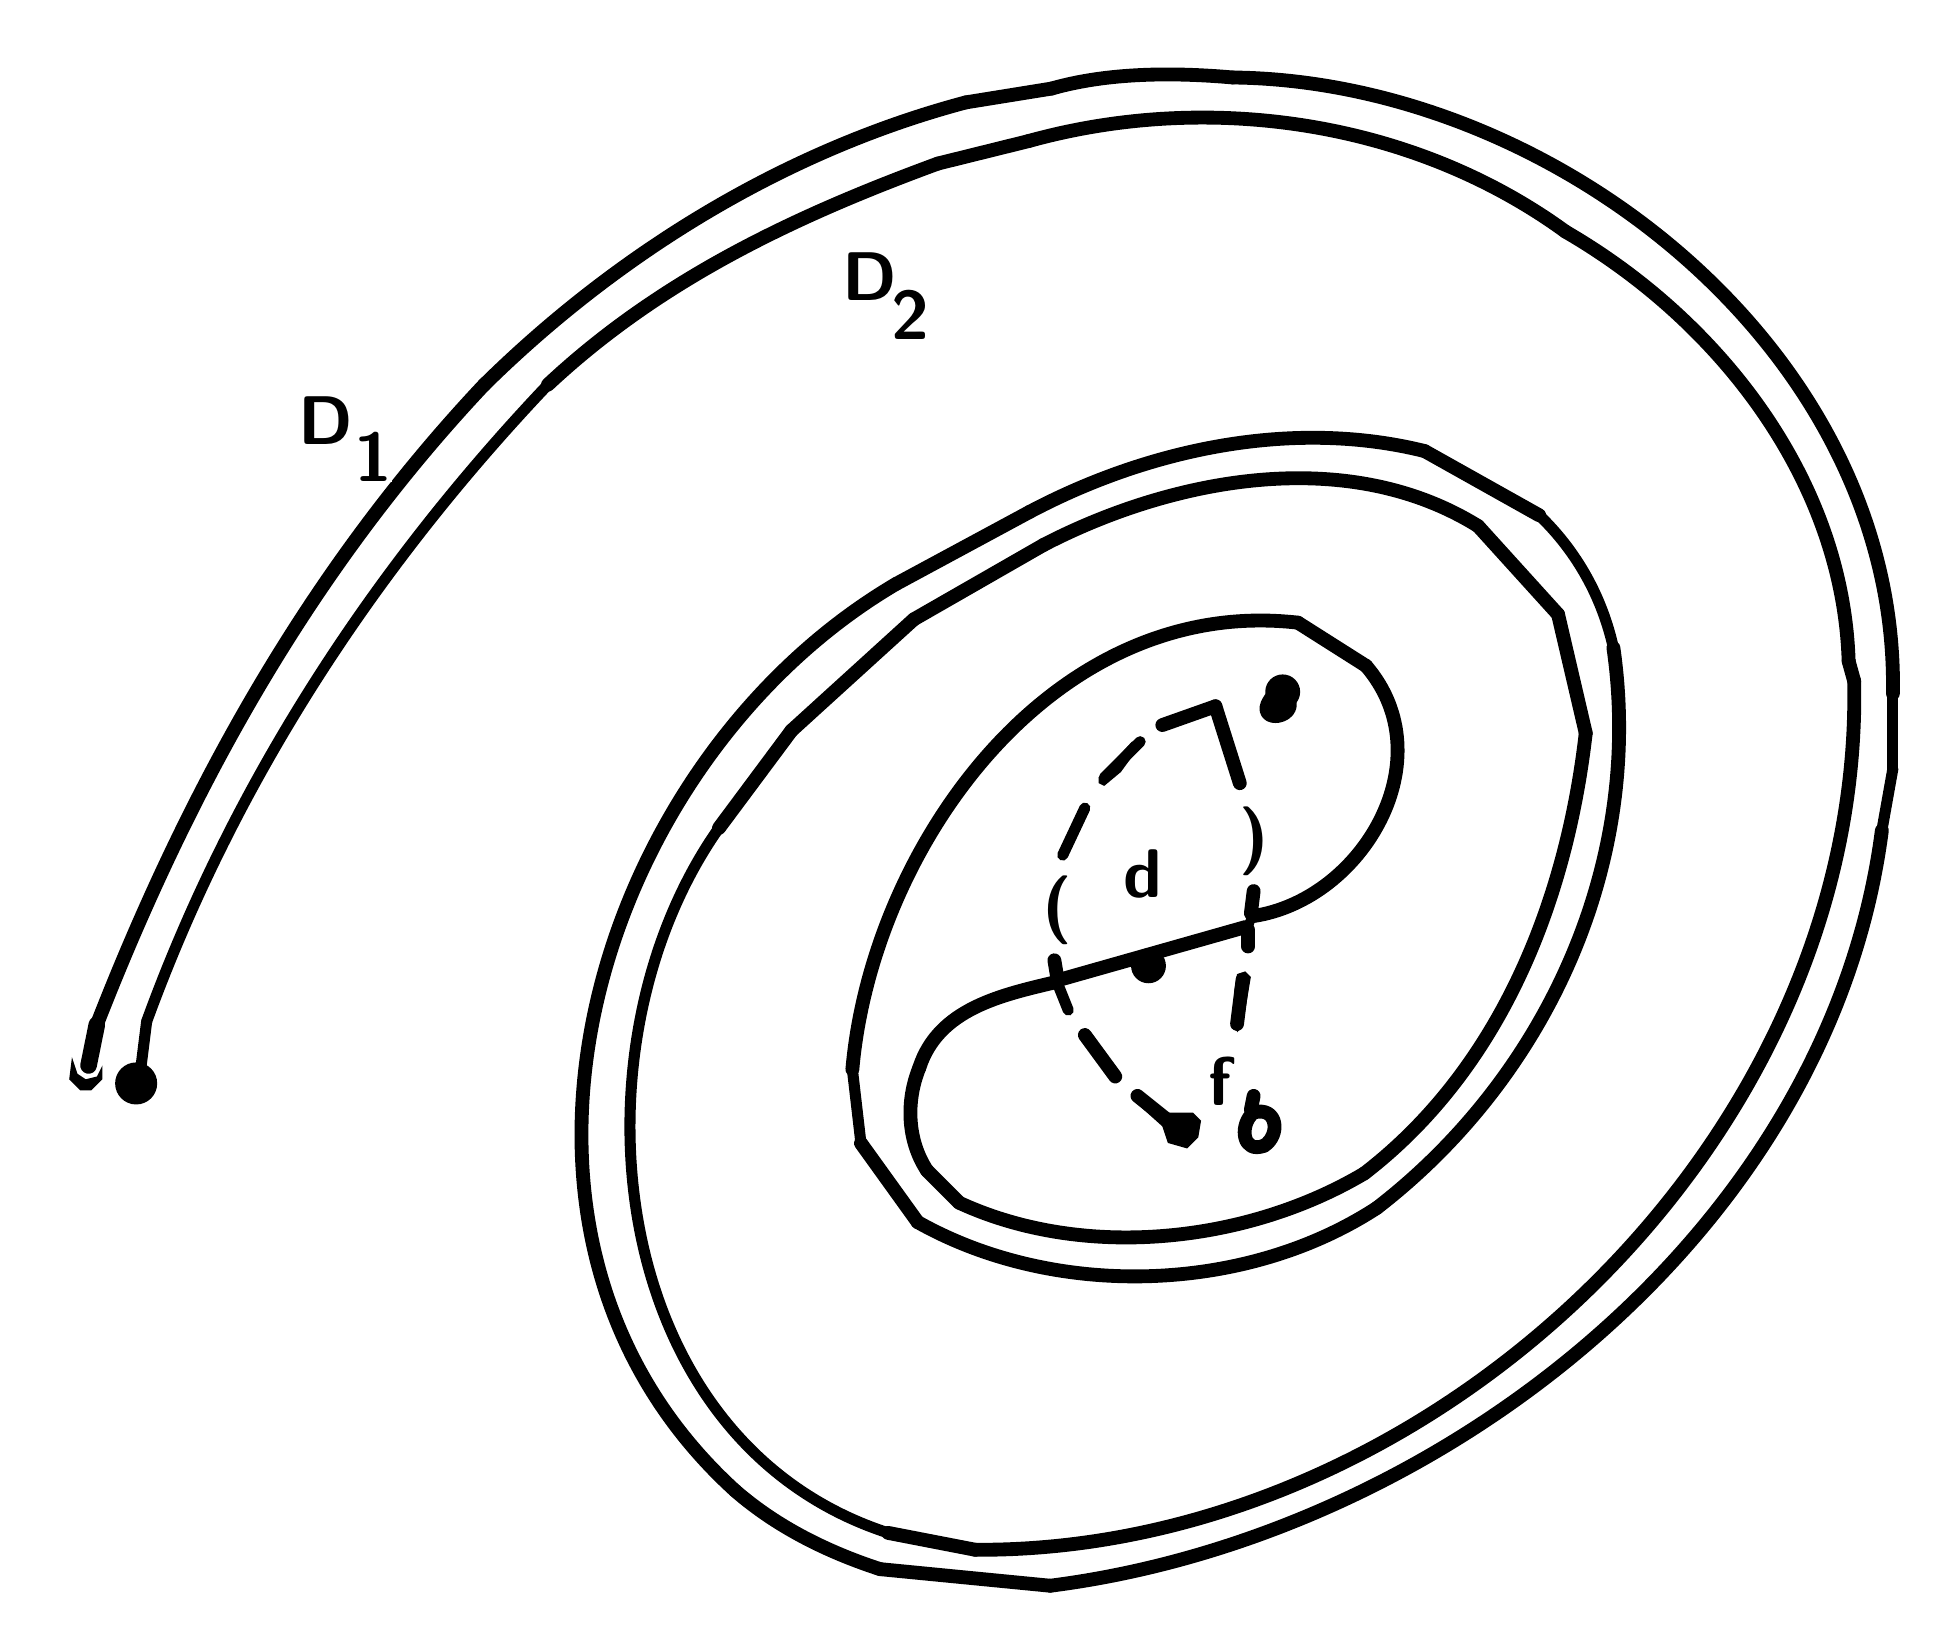
\begin{tikzpicture}[x=1pt, y=-1pt, line width=5.0pt, line cap=round, line join=round]

  %% ════ 填充区（prims2 的 fills）════
  \fill (400.0,385.0) -- (400.0,388.0) -- (410.0,397.0) -- (412.0,403.0) -- (419.0,405.0) -- (423.0,401.0) -- (424.0,395.0) -- (421.0,392.0) -- (411.0,392.0) -- (404.0,386.0) -- cycle;
  \fill (403.0,258.0) -- (399.0,258.0) -- (387.0,271.0) -- (387.0,273.0) -- (389.0,274.0) -- (395.0,269.0) -- cycle;
  \fill (440.0,341.0) -- (437.0,342.0) -- (436.0,348.0) -- (437.0,363.0) -- (439.0,361.0) -- (442.0,343.0) -- cycle;
  \fill (16.0,372.0) -- (15.0,380.0) -- (19.0,384.0) -- (23.0,384.0) -- (27.0,380.0) -- (27.0,375.0) -- (25.0,379.0) -- (21.0,380.0) -- (18.0,378.0) -- cycle;

  %% ════ 直线段（prims2 的 strokes）════
  \draw[line width=5.0pt] (438.0,273.0) -- (429.2,245.2);
  \draw[line width=5.0pt] (429.2,245.2) -- (410.0,252.0);
  \draw[line width=5.0pt] (372.0,343.0) -- (371.0,337.0);
  \draw[line width=4.0pt] (389.0,271.0) -- (402.0,258.0);
  \draw[line width=5.0pt] (373.0,344.0) -- (440.0,325.0);
  \draw[line width=4.0pt] (372.0,345.0) -- (376.0,355.0);
  \draw[line width=6.0pt] (22.0,375.0) -- (25.0,360.2);
  \draw[line width=5.0pt] (339.0,27.0) -- (370.0,22.0);
  \draw[line width=4.0pt] (674.0,240.6) -- (674.0,267.7);
  \draw[line width=4.0pt] (674.0,267.7) -- (670.0,290.1);
  \draw[line width=5.0pt] (369.5,563.0) -- (308.0,557.0);
  \draw[line width=5.0pt] (313.8,201.0) -- (362.0,175.0);
  \draw[line width=5.0pt] (504.8,153.0) -- (546.2,176.2);
  \draw[line width=5.0pt] (321.6,431.6) -- (301.1,403.1);
  \draw[line width=4.0pt] (301.1,403.1) -- (298.0,376.4);
  \draw[line width=5.0pt] (459.0,215.0) -- (483.6,230.6);
  \draw[line width=5.0pt] (382.0,364.0) -- (393.0,379.0);
  \draw[line width=5.0pt] (443.0,386.0) -- (442.0,391.0);
  \draw[line width=5.0pt] (441.0,326.0) -- (441.0,332.0);
  \draw[line width=4.0pt] (374.0,299.0) -- (382.0,282.0);
  \draw[line width=5.0pt] (325.0,413.0) -- (336.6,424.6);
  \draw[line width=5.0pt] (563.0,254.9) -- (553.0,212.0);
  \draw[line width=5.0pt] (553.0,212.0) -- (524.1,180.1);
  \draw[line width=5.0pt] (367.1,186.9) -- (320.2,213.8);
  \draw[line width=5.0pt] (320.2,213.8) -- (276.0,254.0);
  \draw[line width=5.0pt] (276.0,254.0) -- (249.8,289.2);
  \draw[line width=5.0pt] (310.9,543.9) -- (342.4,550.0);
  \draw[line width=5.0pt] (660.0,236.1) -- (658.0,228.9);
  \draw[line width=5.0pt] (361.6,41.0) -- (328.9,49.1);
  \draw[line width=4.0pt] (43.0,359.1) -- (40.0,383.0);
  \draw[line width=5.0pt] (442.0,320.0) -- (443.0,312.0);
  \draw[line width=5.0pt] (439.0,344.0) -- (437.0,360.0);
  \draw[line width=5.0pt] (416.0,398.0) -- (401.0,386.0);
  \draw[line width=3.4pt] (441.0,325.0) -- (442.0,322.0);

  %% ════ 曲线（prims2 的 curves —— 三段式，坐标同为 (y,x)）════
  \draw[line width=5.0pt] (25.0,360.2) .. controls (57.7,276.4) and (101.0,197.0) .. (164.9,129.1);
  \draw[line width=5.0pt] (164.9,129.1) .. controls (213.7,81.0) and (274.2,44.2) .. (339.0,27.0);
  \draw[line width=5.0pt] (370.0,22.0) .. controls (390.2,16.2) and (413.9,16.1) .. (435.5,18.0);
  \draw[line width=5.0pt] (435.5,18.0) .. controls (551.7,19.3) and (676.2,117.0) .. (674.0,240.6);
  \draw[line width=5.0pt] (670.0,290.1) .. controls (651.2,435.5) and (508.9,545.3) .. (369.5,563.0);
  \draw[line width=5.0pt] (308.0,557.0) .. controls (289.3,550.9) and (271.0,542.0) .. (255.7,528.7);
  \draw[line width=5.0pt] (255.7,528.7) .. controls (152.9,435.3) and (204.6,265.2) .. (313.8,201.0);
  \draw[line width=5.0pt] (362.0,175.0) .. controls (404.3,152.6) and (456.5,141.0) .. (504.8,153.0);
  \draw[line width=4.0pt] (546.2,176.2) .. controls (560.1,189.6) and (569.0,206.1) .. (573.0,224.1);
  \draw[line width=5.0pt] (573.0,224.1) .. controls (584.1,300.9) and (549.7,378.5) .. (487.5,426.5);
  \draw[line width=5.0pt] (487.5,426.5) .. controls (439.9,457.5) and (371.2,459.5) .. (321.6,431.6);
  \draw[line width=5.0pt] (298.0,376.4) .. controls (304.9,297.0) and (369.5,204.8) .. (459.0,215.0);
  \draw[line width=5.0pt] (483.6,230.6) .. controls (512.3,264.0) and (482.5,315.0) .. (443.0,321.0);
  \draw[line width=6.0pt] (453.0,240.0) .. controls (463.0,249.1) and (440.4,252.4) .. (451.0,241.0);
  \draw[line width=5.0pt] (442.0,393.0) .. controls (438.1,397.3) and (439.0,406.9) .. (446.8,404.0);
  \draw[line width=5.0pt] (446.8,404.0) .. controls (452.7,400.3) and (451.8,389.6) .. (443.0,392.0);
  \draw[line width=5.0pt] (371.0,345.0) .. controls (352.2,349.5) and (329.1,354.4) .. (322.2,375.8);
  \draw[line width=5.0pt] (322.2,375.8) .. controls (317.3,387.8) and (317.8,402.1) .. (325.0,413.0);
  \draw[line width=5.0pt] (336.6,424.6) .. controls (382.1,445.6) and (440.9,439.0) .. (483.0,414.0);
  \draw[line width=5.0pt] (483.0,414.0) .. controls (533.1,375.4) and (556.2,314.2) .. (563.0,254.9);
  \draw[line width=5.0pt] (524.1,180.1) .. controls (476.5,150.5) and (413.2,163.0) .. (367.1,186.9);
  \draw[line width=4.0pt] (249.8,289.2) .. controls (194.3,367.9) and (208.1,510.5) .. (310.9,543.9);
  \draw[line width=5.0pt] (342.4,550.0) .. controls (506.3,551.1) and (663.4,402.9) .. (660.0,236.1);
  \draw[line width=5.0pt] (658.0,228.9) .. controls (656.0,163.7) and (611.6,106.1) .. (555.7,73.7);
  \draw[line width=5.0pt] (555.7,73.7) .. controls (500.9,33.8) and (427.1,22.8) .. (361.6,41.0);
  \draw[line width=5.0pt] (328.9,49.1) .. controls (278.3,67.7) and (229.1,90.5) .. (188.0,129.0);
  \draw[line width=4.0pt] (188.0,129.0) .. controls (123.6,196.9) and (73.9,274.3) .. (43.0,359.1);

  %% ════ 实心点 ════
  \fill (453.5,240.0) circle (6.3);
  \fill (405.0,339.0) circle (6.3);
  \fill (39.2,381.5) circle (7.6);

  %% ════ 标签（probe 直接给的 \node 行）════
  %% ⚠ 全部补了 fill=white：文字在最上层，否则与曲线交叉干扰
     \node[anchor=center,inner sep=0pt,fill=white,font=\fontsize{30.4}{38.0}\selectfont] at (304.3,90.0) {\textsf{\textbf{\textit{D}}}};   % box(292,79,21,21)
     \node[anchor=center,inner sep=0pt,fill=white,font=\fontsize{23.6}{29.6}\selectfont] at (319.1,103.9) {\textsf{\textbf{2}}};   % box(313,95,11,17)
     \node[anchor=center,inner sep=0pt,fill=white,font=\fontsize{29.6}{37.1}\selectfont] at (107.7,142.0) {\textsf{\textbf{\textit{D}}}};   % box(96,131,20,21)
     \node[anchor=center,inner sep=0pt,fill=white,font=\fontsize{23.7}{29.7}\selectfont] at (124.8,155.4) {\textsf{\textbf{1}}};   % box(118,147,8,16)
     \node[anchor=center,inner sep=0pt,fill=white,font=\fontsize{24.1}{30.1}\selectfont] at (443.2,293.9) {\textsf{\textbf{)}}};   % box(439,282,6,23)
     \node[anchor=center,inner sep=0pt,fill=white,font=\fontsize{30.1}{37.6}\selectfont] at (402.8,305.8) {\textsf{\textbf{\textit{d}}}};   % box(392,294,19,21)
     \node[anchor=center,inner sep=0pt,fill=white,font=\fontsize{26.0}{32.5}\selectfont] at (371.9,318.9) {\textsf{\textbf{(}}};   % box(368,307,7,23)
     \node[anchor=center,inner sep=0pt,fill=white,font=\fontsize{30.2}{37.8}\selectfont] at (432.0,381.0) {\textsf{\textbf{\textit{f}}}};   % box(425,370,13,21)

  % 钉死画布：否则超出的图元/控制点会把页面撑大，1:1 回比就失准
  \pgfresetboundingbox
  \path[use as bounding box] (0,0) rectangle (687,576);
\end{tikzpicture}
\end{document}

% ⚠ 待核清单（probe 拿不准，人眼过一遍）：
%   · 未识别/跳过：⑤ 跳过/未识别的字形
%   · 未识别/跳过：box(409,239,33,36)
%   · 未识别/跳过：box(380,363,16,19)
%   · 未识别/跳过：box(400,385,25,21)
